\section{实时流体模拟算法}
    流体的运动千变万化,通过计算机模拟流体的运动状态是图形学中一个重要的研究课题,它广泛应用于影视、广告、游戏等领域。为了表现复杂灵动的流体,往往需要消耗大量的计算资源,所以实时流体模拟比离线方法更加困难。本文采用了平滑粒子动力学方法进行实时流体模拟,而本章主要阐述了其中压强求解的算法框架,这是保证流体仿真高效、稳定、真实的重要因素。

    \begin{figure}[htbp]
    	\centering
    	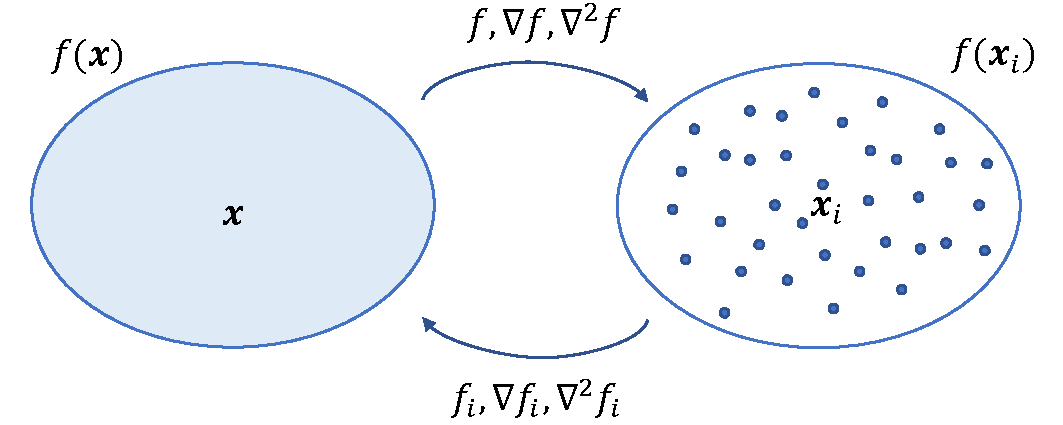
\includegraphics[width=.7\textwidth]{figures/simulation/field.pdf}
    	\caption{SPH物理场离散}
    \end{figure}

\subsection{平滑粒子动力学}
    在宏观尺度的视角下,现实世界的物理现象在空间和时间上都是连续的,为了在计算机上模拟这些现象,首要解决的问题是如何离散这些物理量。在时间上,往往会选择划分为一个个微小时间步,通过显式或隐式时间积分来体现流体的运动。在空间上,可以选择将空间划分为网格或者粒子,它们的区别是网格位置在模拟过程中是不变的,而粒子会随着流体的运动而改变位置。由于粒子之间没有连接关系,所以粒子法比网格法更灵活,更适用于自由表面流体的模拟。

    平滑粒子动力学(SPH)是粒子法的一种,将物理场离散为粒子之后,它通过核函数对离散点积分求得任意位置物理量的近似值(如图\ref{fig:kernelfunc}),而梯度值也可以由核函数梯度积分得到。
    \begin{equation}
    	\begin{gathered}
    	f(\mathbf{x}_i) = \sum_j \frac{m_j}{\rho_j} f(\mathbf{x}_j) W(\mathbf{x}_i - \mathbf{x}_j)
    	\\
    	\nabla f(\mathbf{x}_i) = \sum_j \frac{m_j}{\rho_j} f(\mathbf{x}_j) \nabla W(\mathbf{x}_i - \mathbf{x}_j)
    	\end{gathered}
    \end{equation}
    当 $f$ 为粒子密度时,可以得到流体密度的计算公式
    \begin{equation}\label{eq:densfunc}
    	\rho_i = \sum_j m_j W(\mathbf{x}_i - \mathbf{x}_j)
    \end{equation}
    核函数的定义有许多种,但需要满足以下五个条件:
    \begin{enumerate}
    	\item 归一化条件:$\int_{\mathbb{R}^d} W(\mathbf r, h)\,\mathrm d v = 1$
    	\item 狄拉克$\delta$条件:$\lim_{h\rightarrow 0} W(\mathbf r, h) = \delta (\mathbf r)$
    	\item 非负性条件:$W(\mathbf r, h) \ge 0$
    	\item 对称性条件:$W(\mathbf r, h) = W(\mathbf r, h)$
    	\item 紧支撑条件:$W(\mathbf r, h) = 0 \quad \mathrm{for}\; |\mathbf r| > h$
    \end{enumerate}
    本文中,我们使用Poly6核函数计算一般物理量,而使用Spiky核函数计算物理量梯度\cite{MCG03SPH},定义如下
    \begin{equation}
    	\begin{gathered}
    	W_{\mathrm{Poly6}}(\mathbf r, h) = \frac{315}{64 \pi h^9}
    	\left\{
    	\begin{array}{ll}
    	(h^2 - |\mathbf r|^2)^3 & 0 \le |\mathbf r| < h \\
    	0 & \mathrm{otherwise} \\
    	\end{array}
    	\right.
    	\\
    	\nabla W_{\mathrm{Spiky}}(\mathbf r, h) = -\frac{45}{\pi h^6}
    	\left\{
    	\begin{array}{ll}
    	\frac{\mathbf r}{|\mathbf r|} (h - |\mathbf r|)^2 & 0 < |\mathbf r| < h \\
    	\mathbf 0 & \mathrm{otherwise} \\
    	\end{array}
    	\right.
    	\end{gathered}
    \end{equation}
    其中 $h$ 为核函数支撑域半径,$\mathbf r$ 为采样点到核函数中心的方向向量。
    
    \begin{figure}
    	\centering
    	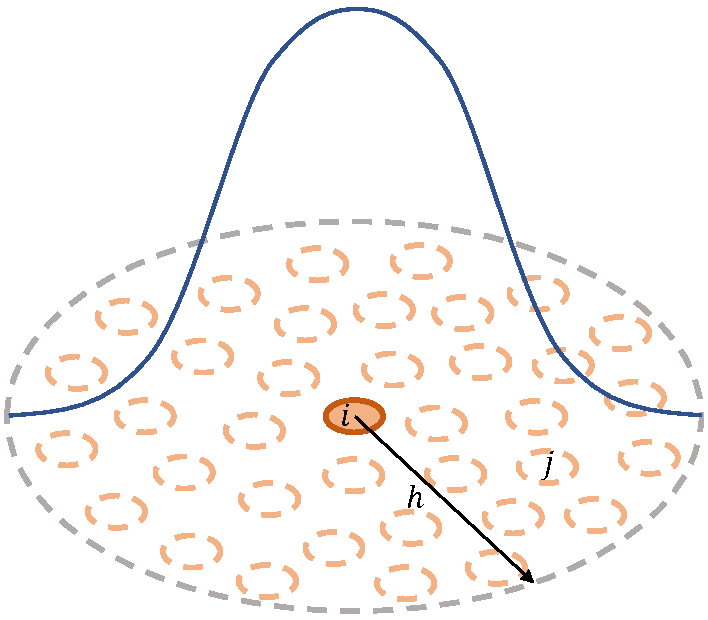
\includegraphics[width=.45\textwidth]{figures/simulation/kernel.pdf}
    	\caption{平滑核估计}
    	\label{fig:kernelfunc}
    \end{figure}
    
    \begin{figure}
    	\centering
    	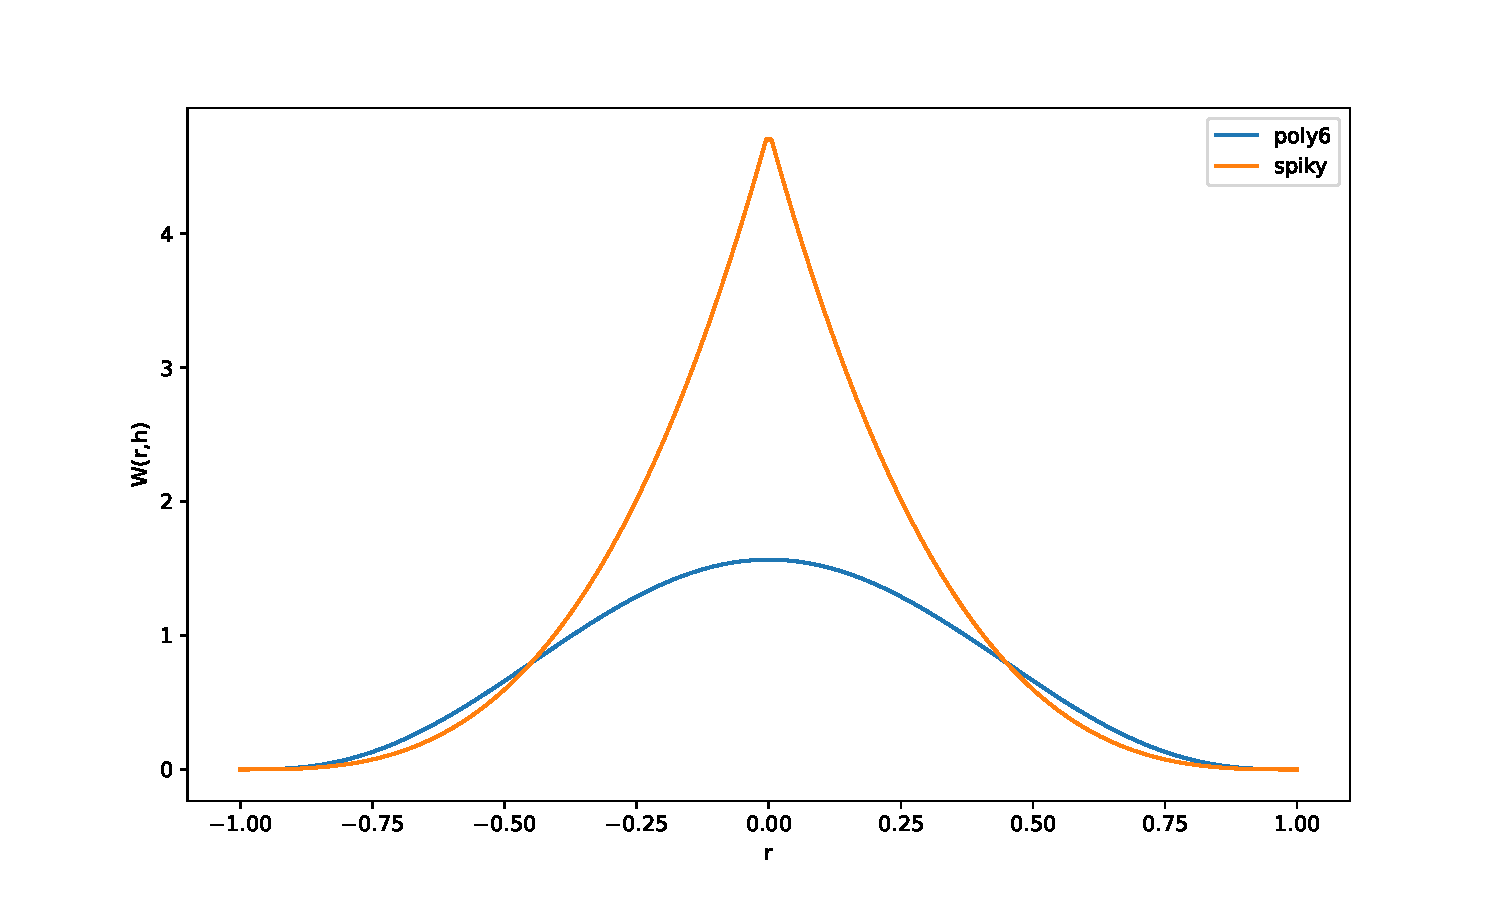
\includegraphics[width=.85\textwidth]{figures/simulation/kernel_func.pdf}
    	\caption{核函数示意图}
    \end{figure}

\subsection{基于位置的流体}
    在表现流体运动状态时,保证不可压缩性是体现流体真实感的关键因素。而不可压缩性在物理上可以描述为速度场旋度为0($\nabla \cdot \mathbf v = 0$),或密度场恒定($\rho = \rho_0$ )。大部分图形学中的模拟方法都是通过这两个条件之一计算流体压强与受力,再通过牛顿第二定律计算加速度,最后通过时间积分得到粒子速度与位置。而Macklin等人\cite{MM13PBF}提出了基于位置的方法(PBF),将不可压缩性条件转化为粒子位置约束,忽略了繁琐的时间积分过程,直接更新粒子位置。这种方法更加高效且容易控制。

\subsubsection{强制不可压缩约束}
    为了满足流体密度恒定的条件,我们需要求解一个非线性的约束 $\mathbf C$,且在每个流体粒子上都存在一个约束 $C_i$。每个约束都可以写成粒子位置及其近邻粒子位置的函数,根据密度计算公式\ref{eq:densfunc},我们可以将第 $i$ 个粒子的约束状态表示为
    \begin{equation}
    	C_i(\mathbf{x}_1,...,\mathbf{x}_n)  = \frac {\rho_i} {\rho_0} - 1
    \end{equation}
    其中 $\rho_0$ 为初始状态流体密度。我们的求解目标是对每个粒子寻找一个位置更新向量 $\Delta \mathbf x_i$,使得所有约束条件都满足 $C_i(\mathbf x + \Delta \mathbf x_i) = 0$。那么对于整个约束系统就意味着
    \begin{equation}\label{eq:constrainsys}
    	\mathbf C(\mathbf x + \Delta \mathbf x) = \mathbf 0
    \end{equation}
    这个非线性约系统显然难以直接求解,所以我们使用牛顿法迭代优化的思想,每次迭代沿着位置约束函数的梯度方向更新位置,设更新步长为 $\lambda$,则
    \begin{equation}
    	\Delta \mathbf x = \nabla \mathbf C(x) \lambda
    \end{equation}
    进一步对公式\ref{eq:constrainsys}进行泰勒展开,可以得到:
    \begin{equation}
    	\begin{aligned}
    	\mathbf C(\mathbf x + \Delta \mathbf x) 
    	& \approx \mathbf C (\mathbf x) + \nabla \mathbf C^T(\mathbf x) \Delta \mathbf x \\
    	& \approx \mathbf C (\mathbf x) + \nabla \mathbf C^T(\mathbf x) \nabla \mathbf C(\mathbf x) \lambda = 0 \\
    	\end{aligned}
    \end{equation}
    在泰勒展开后忽略高阶项,我们的目标是使得约束为零,则可以利用这个条件反过来求得更新步长
    \begin{equation}\label{eq:lambda1}
    	\begin{gathered}
    	\lambda = - \frac {\mathbf C (\mathbf x)} {\nabla \mathbf C^T(\mathbf x) \nabla \mathbf C(\mathbf x)} \\
    	\lambda_i = - \frac {C_i} {\sum_k |\nabla_k C_i|^2}
    	\end{gathered}
    \end{equation}


\subsubsection{更新步长与位置更新向量}
    上文推导了PBF是如何迭代求解约束系统(公式\ref{eq:constrainsys})的,接下来我们需要具体推导每次迭代中更新步长和位置更新向量的计算公式。

    第一节公式\ref{eq:ns1}介绍了如何SPH方法如何计算物理场及其梯度,我们可以按照同样的方法计算约束函数的梯度。具体地,约束 $C_i$ 对粒子 $k$ 梯度如下式所示,需要注意的是,某粒子对应的约束对其本身球梯度或是对其近邻粒子求梯度,计算公式是不同的。
    \begin{equation}
    	\begin{aligned}
    	\nabla_k C_i &= \frac {1} {\rho_0} \sum_j m_j \nabla_k W_{ij} \\
    	&=
    	\frac {1} {\rho_0}
    	\left\{
    	\begin{array}{ll}
    	\sum_j m_j \nabla W_{ij} & \mathrm{if} \ k = i \\
    	-m_j \nabla W_{ij} & \mathrm{if} \ k = j \\
    	\end{array}
    	\right.
    	\\
    	\end{aligned}
    \end{equation}
    将其代入公式\ref{eq:lambda1},可得 $\lambda_i$ 的具体计算公式为
    \begin{equation}\label{eq:lambda2}
    	\lambda_i = - \frac 
    	{ \max(\frac{\rho_i} {\rho_0} - 1, 0) } 
    	{ \frac {1}{\rho_0^2} (|\sum_j m_j \nabla W_{ij}|^2 + \sum_j |m_j \nabla W_{ij}|^2 ) + \varepsilon }
    \end{equation}
    
    由于公式\ref{eq:constrainsys}是非线性的,并且在核函数逼近其边界时梯度非常小,所以公式\ref{eq:lambda1}的分母会在粒子间距逼近核函数半径时造成整个系统的不稳定。因此我们在公式\ref{eq:lambda2}的分母中引入松弛参数 $\varepsilon$ 防止计算崩溃。这相当于正则化约束函数,即
    \begin{equation}
    	\mathbf C(\mathbf x + \Delta \mathbf x) 
    	\approx \mathbf C (\mathbf x) + \nabla \mathbf C^T(\mathbf x) \nabla \mathbf C(\mathbf x) \lambda + \varepsilon \lambda = 0
    \end{equation}

    最后,在得到更新步长之后,可以计算位置更新向量
    \begin{equation}
    	\Delta \mathbf x_i = \lambda_i \nabla_iC_i = 2\lambda_i \frac{1}{2\rho_0} \sum_j m_j \nabla W_{ij} \approx
    	\frac{1}{2\rho_0} \sum_j (m_i \lambda_i + m_j \lambda_j) \nabla W_{ij}
    \end{equation}
    
    SPH流体模拟通常会由于粒子没有足够的临近粒子,局部无法满足密度恒定约束从而产生负压强,导致粒子过度聚集。Macklin等人引入了人工压强项\cite{M00SPH}防止这一现象,同时模拟了表面张力效果。不过这并不是物理正确的,需要调整参数在缓解粒子聚集和表面张力效果之间寻找一个平衡点。而本文中直接不考虑负压强的影响(公式ref{eq:lambda2}分子),同时在仿真框架中引入表面张力模型,计算物理正确的粒子间内聚力与表面张力。表面张力建模将在第四章中详细阐述。

\subsection{边界条件}

    上文描述了流体粒子之间的运动状态求解,但是流体不可能在一个无限的空间中运动,所以需要确定流体粒子如何与固体边界进行交互。本节仅考虑流体与固体单向耦合,即固体是静态的,不会由于流体碰撞而发生移动。PBF框架是完全基于位置计算密度约束的,所以可以直接改变粒子位置使其满足边界条件,即在更新粒子位置时判断其是否超出了边界范围,如果超出边界则直接将其位置改变至边界内部。
    
    这种方法简单有效,但不是物理正确的,这会导致边界处粒子欠采样,而为了满足密度约束,会有大量粒子聚集在边界附近。一种常用的解决方法是将固体边界也离散化为粒子\cite{AIA12SPHB},将固体粒子也参与到流体粒子的密度计算和压强计算中来。但是这种方法消耗存储空间较大,且边界越复杂固体粒子越多需要离散的精度也越高。由于浏览器端资源空间受限,本文所实现的流体仿真框架所支持的最高粒子数为256k(详见5.3.4节), 使用固体粒子的方法虽然简单但是会大大压缩流体粒子的数量,降低流体仿真的真实感。所以本文采用Bender等人\cite{BKW19SPHB}提出的边界体积贴图(Volume Map)方法,这是一种隐式的边界表示方法,需要预计算空间每处边界固体的体积,而后在实时仿真中就可以通过贴图的方式高效查找。在原理上,体积贴图(Density Map)\cite{KB17SPHB}是密度贴图的改进方法,所以本文将先介绍密度贴图方法,再介绍体积贴图的改进点与具体实现。
    
    \begin{figure}
    	\centering
    	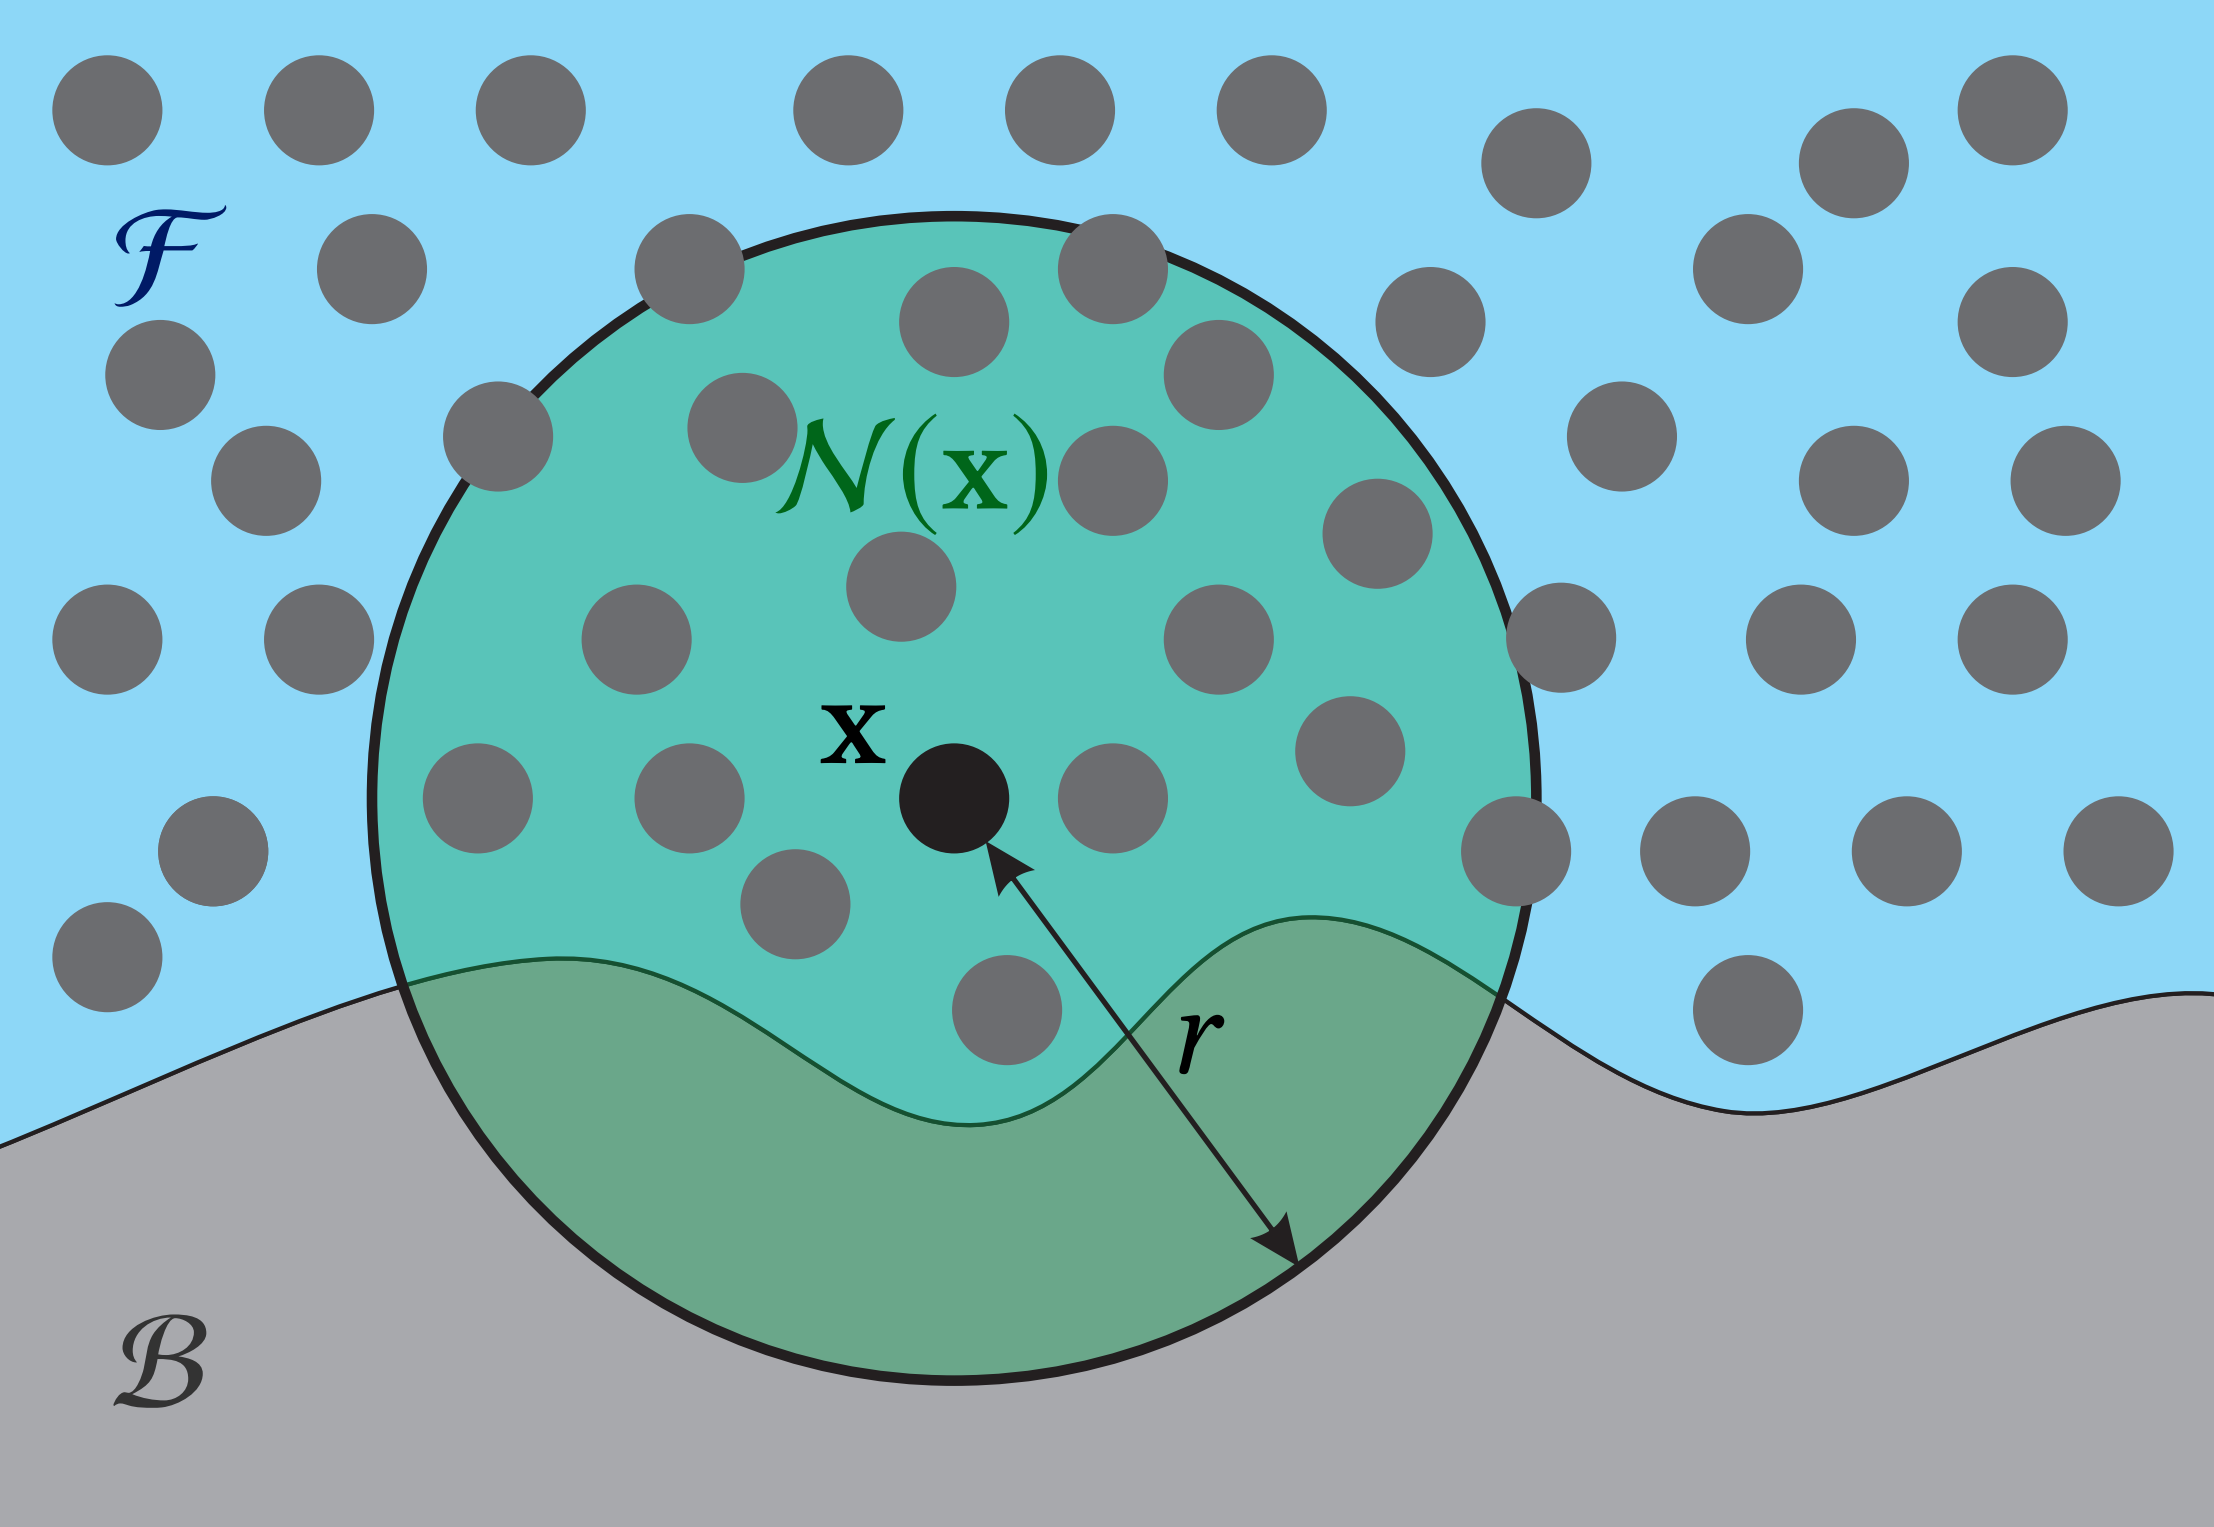
\includegraphics[width=.55\textwidth]{figures/simulation/boundary.png}
    	\caption{边界条件($\mathcal F$ 为流体,$\mathcal B$ 为固体边界,$\mathcal N(\mathbf x)$ 为粒子 $\mathbf x$ 的邻域)}
    \end{figure}

\subsubsection{密度贴图}

    公式\ref{eq:densfunc}描述了流体密度的计算公式,其在流体内部是正确的,但是在边界处由于未考虑边界固体的密度贡献从而造成欠采样,如果加上这部分贡献,密度计算公式可以表示为
    \begin{equation}\label{eq:densfuncb}
    	\begin{aligned}
    	\rho(\mathbf x) &=
    	\int_{\mathcal N (x) \cap \mathcal F} \rho(\mathbf x') W(\mathbf{x} - \mathbf{x}')\, \mathrm d \mathbf x'
    	+
    	\int_{\mathcal N (x) \cap \mathcal B} \rho(\mathbf x') W(\mathbf{x} - \mathbf{x}')\, \mathrm d \mathbf x'
    	\\
    	&= \rho_{\mathcal F}(\mathbf x) + \rho_{\mathcal B}(\mathbf x)
    	\end{aligned}
    \end{equation}
    而在具体计算边界密度贡献 $\rho_{\mathcal B}$ 时,将固体密度等同于流体初始密度 $\rho_0$,
    \begin{equation}
    	\begin{gathered}
    	\rho_{\mathcal B}(\mathbf x) =
    	\int_{\mathcal N(\mathbf x)} \phi (D(\mathbf x')) W(\mathbf{x} - \mathbf{x}') \, \mathrm d \mathbf x'
    	\\
    	\phi(d) = 
    	\left\{
    	\begin{array}{ll}
    	\rho_0 (1 - \frac {d}{h}) & \mathrm{if} \; d < h \\
    	0 & \mathrm{otherwise}
    	\end{array}
    	\right.
    	\end{gathered}
    \end{equation}
    其中 $D(\mathbf x)$ 为有向距离函数,表示 $\mathbf x$ 到边界的最短距离,如果为负值则表示 $\mathbf x$ 在固体内部,为正值则表示在固体外部流体内部。而 $\phi(d)$ 是一个简单的线性平滑函数,他将固体边界的密度影响向外扩大了 $h$,防止密度值在边界上突变。

\subsubsection{体积贴图}

    通过公式\ref{eq:densfuncb}可以很直观的计算空间各处边界固体对流体粒子的密度贡献,但是SPH模型往往要通过密度的梯度计算压强,而通过公式\ref{eq:densfuncb}计算密度梯度就相当于对核函数梯度进行积分,这会导致梯度方向计算产生误差,所以Bender等人\cite{BKW19SPHB}提出了体积贴图方法,不再计算边界密度贡献,而是计算边界体积
    \begin{equation}
    	\begin{gathered}
    	V_{\mathcal B} (\mathbf x) = 
    	\int_{\mathcal N(\mathbf x)} \phi^* (D(\mathbf x')) \, \mathrm d \mathbf x' 
    	\\
    	\phi^*(d) = 
    	\left\{
    	\begin{array}{ll}
    	\frac{W_{cubic}(d)}{W_{cubic}(0)} & \mathrm{if} \; 0 < d < h \\
    	1 & \mathrm{if} \; d \le 0 \\
    	0 & \mathrm{otherwise} \\
    	\end{array}
    	\right.
    	\end{gathered}
    \end{equation}
    体积贴图使用的平滑函数 $\phi^*$ 的定义与密度贴图的计算略有不同,式中 $W_{cubic}$ 表示三阶样条核函数\cite{MCG03SPH}。在具体实现上,我们使用高斯-勒让德积分(Gauss-Legendre quadrature)数值求解公式积分值。而针对有向距离函数 $D$ ,我们则使用了Bærentzen等人\cite{BH05SDF}提出的有向距离场(Signed Distance Field, SDF)计算方法,对SDF插值即可得到空间中任意位置的有向距离,针对SDF的空间离散与插值方法与体积贴图相同,将在3.3.3节具体介绍。我们在确定了边界体积的大小之后,可以很容易地确定边界密度的对流体粒子 $\mathbf x$ 的贡献
    \begin{equation}
    	\rho_{\mathcal B}(\mathbf x) =
    	V_{\mathcal B} (\mathbf x) \rho_0 W(\mathbf x - \mathbf x^*)
    \end{equation}
    上式中 $\mathbf x^*$ 是距离 $\mathbf x$ 最近的边界点,可以由SDF反推得知。
    
    结合上一节中阐述的PBF流体仿真算法,可以将边界密度贡献添加到PBF的密度约束中(公式\ref{eq:constrainsys}),这样 $\lambda_i$ 的计算公式(公式\ref{eq:lambda2})就变为了
    \begin{equation}
    	\lambda_i = - \frac 
    	{ \max(\rho_i^{\mathcal F} / \rho_0 + V_i^{\mathcal B} W(\mathbf x_i - \mathbf x_i^*) - 1, 0) }
    	{ \frac {1}{\rho_0^2} (|\sum_j m_j \nabla W_{ij}|^2 + \sum_j |m_j \nabla W_{ij}|^2 ) + \varepsilon }
    \end{equation}
    同样可以得到边界条件对PBF中位置更新向量的影响为
    \begin{equation}
    	\Delta \mathbf x_{\mathcal B} = \frac{1}{2} \lambda_i V_{\mathcal B}(\mathbf x) \nabla W(\mathbf x - \mathbf x^*)
    \end{equation}
    则加入边界条件影响的位置更新向量计算公式会变为
    \begin{equation}
    	\Delta \mathbf x_i \approx
    	\frac{1}{2\rho_0} \sum_j (m_i \lambda_i + m_j \lambda_j) \nabla W_{ij} +
    	\frac{1}{2} \lambda_i V_i^{\mathcal B} \nabla W(\mathbf x_i - \mathbf x_i^*)
    \end{equation}
    
    \begin{figure}
    	\centering
    	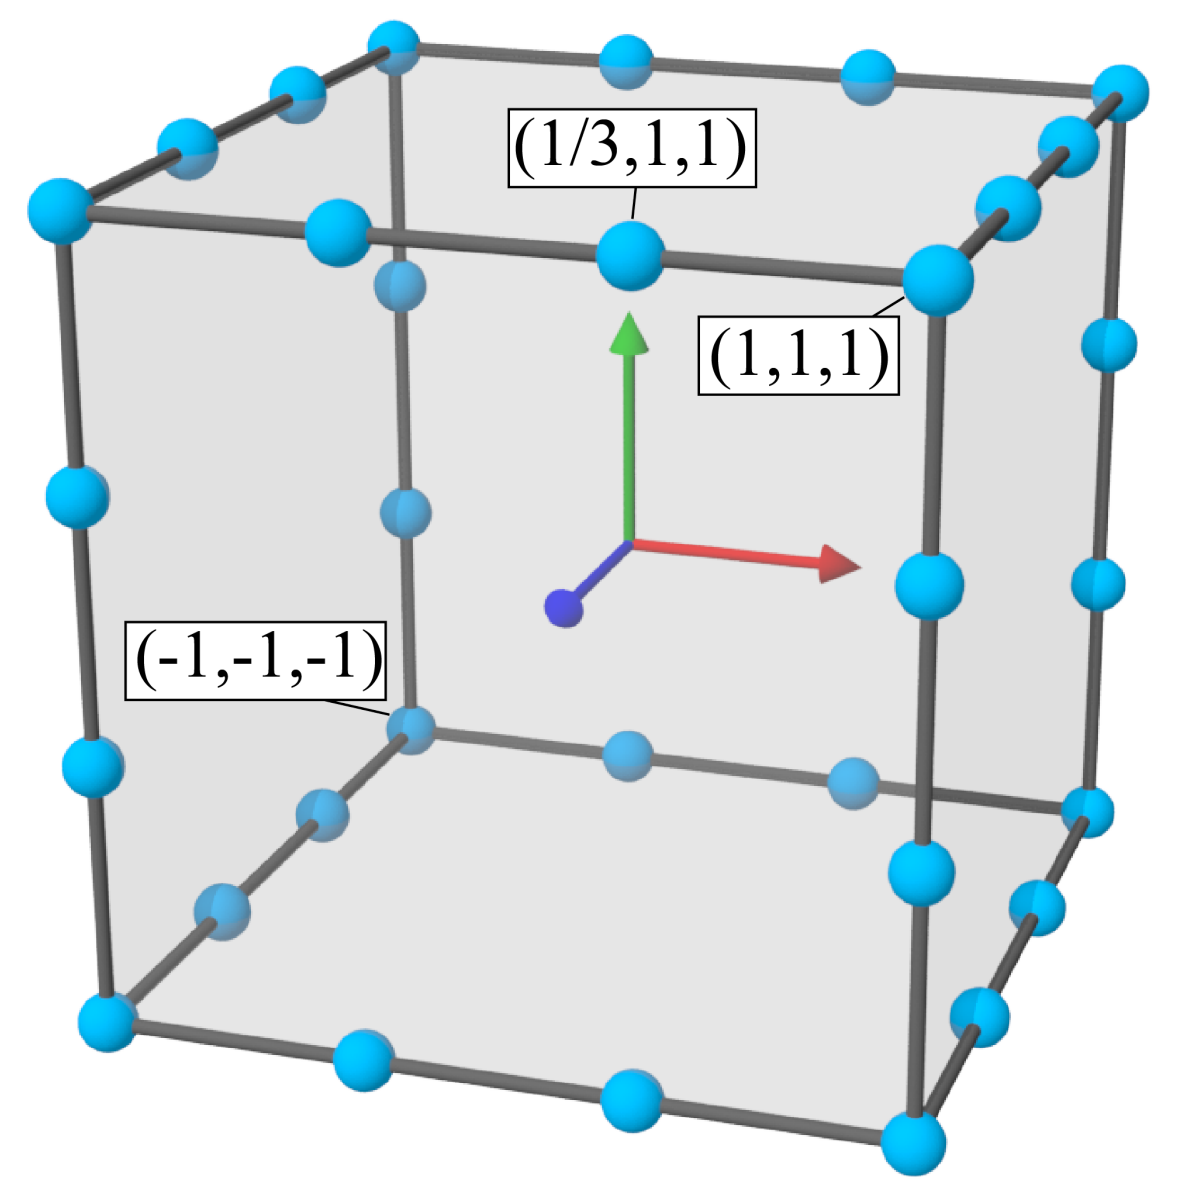
\includegraphics[width=.4\textwidth]{figures/simulation/sample.png}
    	\caption{三次多项式插值}
    	\label{fig:cubicsample}
    \end{figure}

\subsubsection{空间离散}
    在具体实现上,本文使用六面体网格划分空间,并采用Bender等人\cite{BKW19SPHB}推荐的Serendipity类型三次多项式离散化边界体积。查询空间中任意位置的边界体积值需要插值32个采样点(如图\ref{fig:cubicsample})。插值函数定义如下:
    \begin{equation}\label{eq:samplefunc}
    	f(\mathbf x') \approx \sum_{i=1}^{32} w_i(\mathbf x') s_i \qquad \mathbf x' \in [-1,1]^3 
    \end{equation}
    在插值计算时需要注意,要先将粒子位置转换到以六面体网格为中心的局部坐标中,具体计算方式为 $\mathbf x' = [\mathrm{diag}(\mathbf b - \mathbf a)]^{-1}(2\mathbf x -(\mathbf a + \mathbf b))$,$\mathbf a,\; \mathbf b$分别为此六面体最大和最小格点位置。公式\ref{eq:samplefunc}中 $s_i$ 为采样点数据,$w_i$ 为型函数(Shape Function),其计算结果为插值权重,定义如下
    \begin{equation}
    	w_i(\mathbf x) =
    	\left\{
    	\begin{array}{lll}
    
    	\frac{1}{64} (1 + \xi x)(1 + \eta y)(1 + \zeta z) \left[ 9(x^2 + y^2 + z^2)-19 \right] 
    	& \mathrm{corner} & (\xi,\eta,\zeta=\pm 1) \\
    
    	\frac{9}{64} (1 - x^2) (1 + 9 \xi x) (1 + \eta y) (1 + \zeta z)
    	& x\; \mathrm{edge} & (\xi=\pm \frac{1}{3} \quad \eta,\zeta=\pm 1) \\
    
    	\frac{9}{64} (1 - y^2) (1 + \xi x) (1 + 9 \eta y) (1 + \zeta z)
    	& y\; \mathrm{edge} & (\eta=\pm \frac{1}{3} \quad \xi,\zeta=\pm 1)\\
    
    	\frac{9}{64} (1 - z^2) (1 + \xi x) (1 + \eta y) (1 + 9 \zeta z)
    	& z\; \mathrm{edge} & (\zeta=\pm \frac{1}{3} \quad \xi,\eta=\pm 1) \\
    
    	\end{array}
    	\right.
    \end{equation}
    其中 $(\xi,\,\eta,\,\zeta)$ 为采样点坐标。
    
    \begin{figure}
    	\centering
    	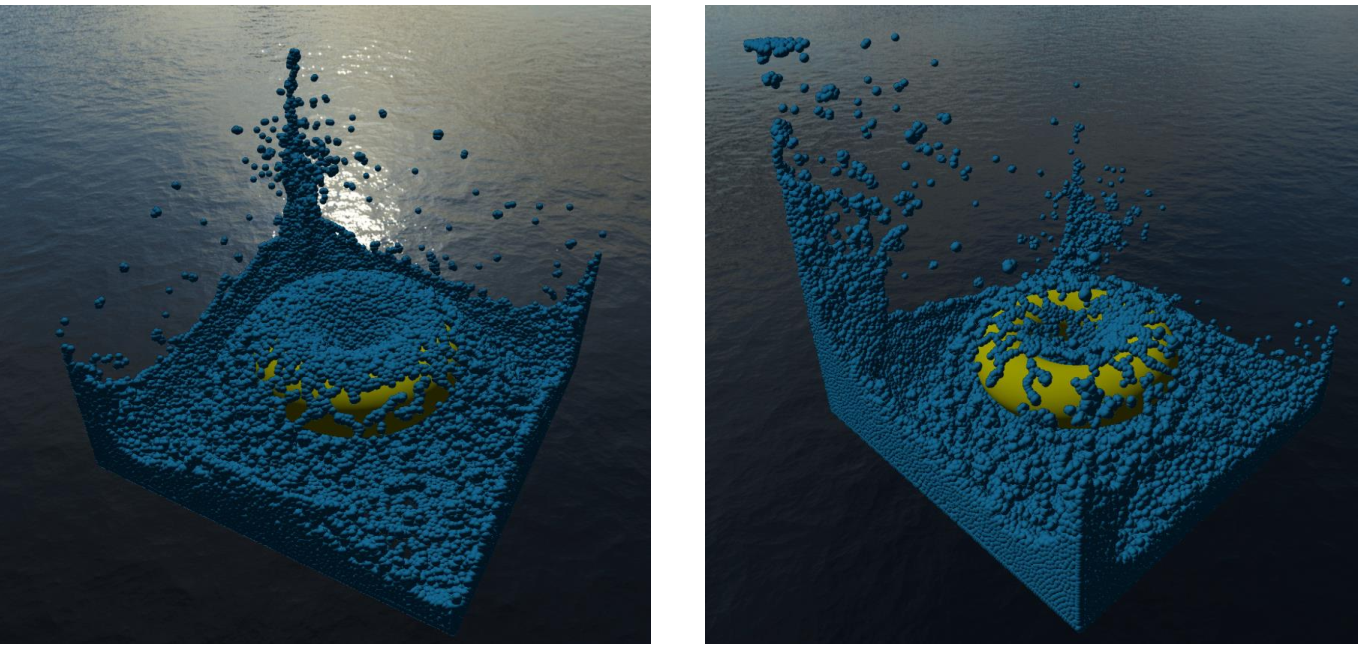
\includegraphics[width=.95\textwidth]{figures/simulation/boundary_sample.pdf}
    	\caption{固体圆环边界与流体粒子交互}
    \end{figure}

\subsection{本章小结}
    本章主要阐述了不可压缩流体的模拟算法。首先介绍了SPH方法,如何从粒子视角离散近似物理场及其梯度场。接下来以基于位置的动力学的思想为基础,推导了PBF在密度恒定约束下的粒子位置迭代公式。最后介绍了一种隐式边界条件表示方法——体积贴图法,并将其添加到PBF的框架中。总的来说,本章的核心是PBF,一种直接改变粒子位置的迭代式压强求解方法,它稳定且高效,适用于实时不可压缩流体仿真。